\begin{center}

  \begin{tabular}{rp{16cm}lp{20cm}}%{rl}

  % after \\: \hline or \cline{col1-col2} \cline{col3-col4} ...

  论文地址:& \href{https://arxiv.org/pdf/1505.04597.pdf}{https://arxiv.org/pdf/1505.04597.pdf} \\
  来源:& LNCS, 2015 \\
  作者:& Ronneberger, Olaf and Fischer, et al. \\

  %源码:& \href{xxx}{xxx} \\

%  slides:& \href{http://yunshengb.com/wp-content/uploads/2017/03/nips_2018_r2l_workshop_talk.pdf}{{\footnotesize Convolutional Set Matching for Graph Similarity}}\\

  关键词:& \textbf{Image Segmentation, Bimedical Image} \\

  写于:& \date{2021-04-19}

  \end{tabular}

\end{center}

该论文\cite{ronneberger2015u-net}提出的U-Net,是较早将卷积神经网络应用到图像语义分割的模型。U-Net是在FCN\cite{long2015fully}的基础上构建的。U-Net包含contracting path来提取图像特征/上下文、expanding path来进行精确的分割。

\paragraph{Motivation}
CNN通常用被用于分类,并且需要大量的数据。然而在医学图像处理任务中,不仅仅是对图像分类,还需要对图像进行逐像素的分割,而且通常无法获得大量的医学图像数据。在之前的一些方法中,将像素周围的局部区域划分为一个patch来预测一个像素的类别,这样获得的patch的数量远远大于图像的数量。但是这种方法有两个明显的缺点:1)速度慢,因为需要单独计算每个patch来预测像素类别,而且patch之间存在巨大的冗余;2)预测的准确率受所使用的patch的size的影响。还有一些方法使用不同层级的feature map来进行分割(如金字塔模型)。

鉴于已有方法的缺陷,U-Net在FCN\cite{long2015fully}的基础上进行修改和扩充,使得U-Net能够在数据量小的情况下得到更好的、高精度的分割效果。

\paragraph{U-Net}
U-Net结构如Fig.\ref{fig:unet}所示。
\begin{figure}[h]
	\centering
	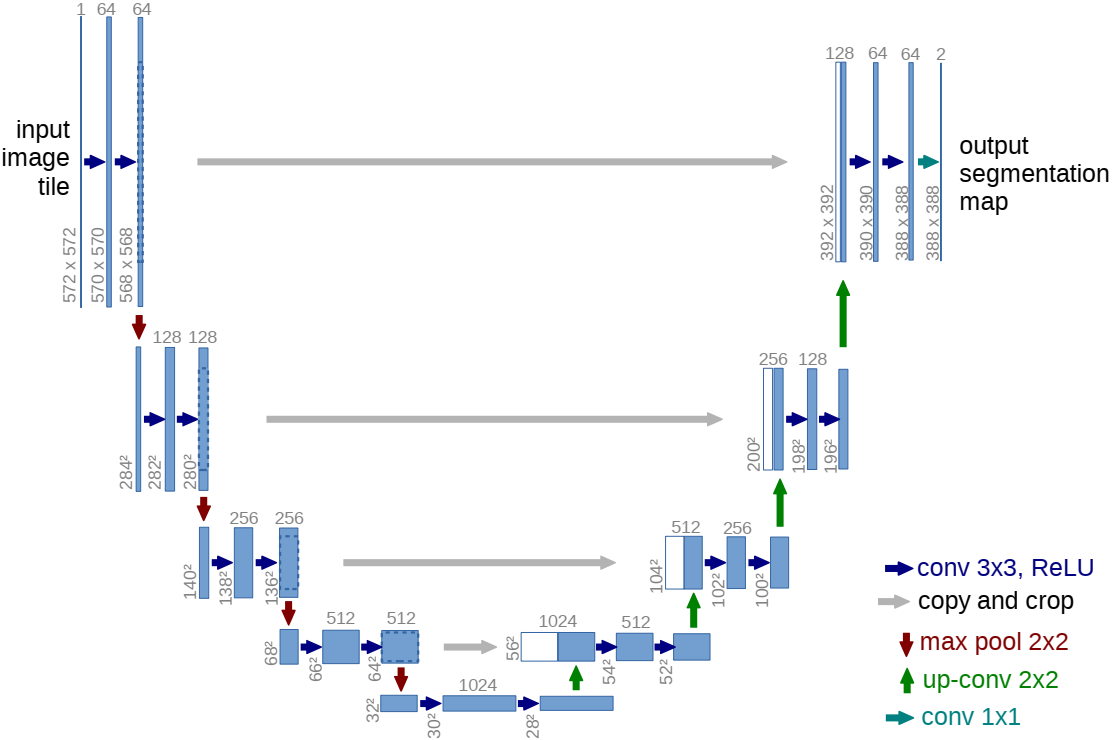
\includegraphics[width=.8\textwidth]{pics/unet.png}
	\caption{U-Net architecture}
	\label{fig:unet}
\end{figure}
U-Net整体可以分为两部分,左边的压缩路径部分和右边的扩展路径部分。

在压缩路径上,输入的源图像经过卷积、max-pooling,尺寸逐渐变小,尺寸每为原来的二分之一,通道数则变为原来的两倍。在扩展路径上,feature map经过up-conv、卷积,尺寸逐渐增大,尺寸每变为原来的两倍,通道数变为原来的二分之一。除了左右两边的路径,U-Net还会将左边的压缩路径上的feature map裁剪一部分与右边的扩张路径同层级的feature map在通道上进行拼接,如Fig.\ref{fig:unet}中间灰色箭头所示。

到目前为止,U-Net都是比较简洁明了的,现在来更深入地挖掘一下。

\par{\textbf{Overlap-tile strategy}} 使用U-Net对源图像进行分割时,我们可以看到输出的分割结果比源图像要小,为了使得U-Net能够对任意大小的图像进行无缝的(seamless)分割,U-Net使用了Overlap-tile strategy,如Fig.\ref{fig:overlap-tile}所示。
\begin{figure}[h]
	\centering
	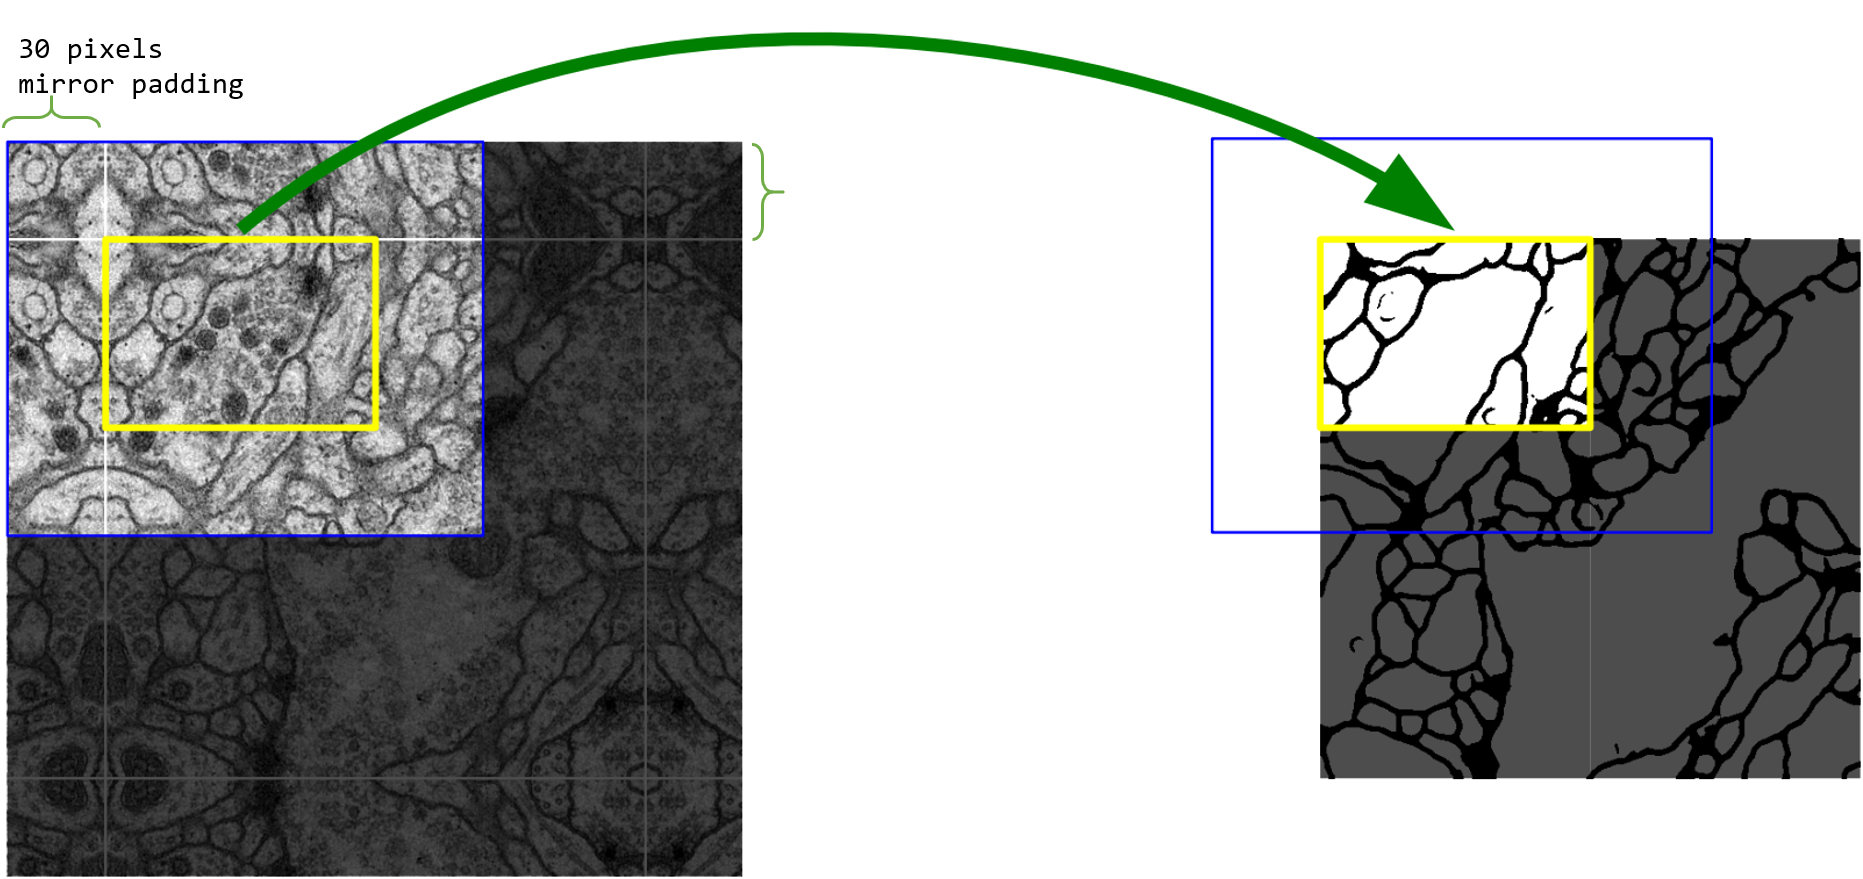
\includegraphics[width=.8\textwidth]{pics/Overlap-tile strategy.png}
	\caption{Overlap-tile strategy}
	\label{fig:overlap-tile}
\end{figure}
对于很大的图像,进行分割时可能需要将其进行划分成符合网络输入的块,原本在源图像内处于内部的区域可能成为了块的边界,在对块进行分割时,可能会产生缝隙/无法与相邻块的分割结果对齐。为了解决这个问题,也为了维持分割结果的size,U-Net使用了Overlap-tile strategy,以块的边界为轴进行镜像对称来对块进行padding(这一点不是很确定,论文中原文是:\textit{only use the valid part of each convolution})。

\par{\textbf{损失函数}}
为了让U-Net对边界有更好的分割效果、对与相邻的同类区域也有较好的分割效果,U-Net使用了带权重的交叉熵损失函数,该损失函数在每个像素处对$p_{l(\boldsymbol{x})}(\boldsymbol{x})$与1的偏差进行了惩罚:
$$
E = \sum_{\boldsymbol{x} \in \omega} w(\boldsymbol{x}) log(p_{l(\boldsymbol{x})}(\boldsymbol{x}))
$$
其中$\boldsymbol{x} \in \Omega, \Omega \subsxet \mathbb{Z}^2$,$\boldsymbol{x}$表示像素位置,$l: \Omega \rightarrow {1, ..., K}$表示每个像素的真实标签。$p_{l(\boldsymbol{x})}$是$softmax$函数,$w: \Omega \rightarrow \mathbb{R}$表示像素的权重。使用$w$有两个原因:1)类别不平衡;2)强调分割边界。$w$定义如下:
$$
w(\boldsymbol{x}) = w_c(\boldsymbol{x}) + w_0 \cdot exp(-\frac{(d_1(\boldsymbol{x}) + d_2(\boldsymbol{x}))^2}{2\sigma^2})
$$
其中$w_c: \Omega \rightarrow \mathbb{R}$用于解决类别不平衡的问题,$d_1: \Omega \rightarrow \mathbb{R}$表示$\boldsymbol{x}$到最近的细胞的距离(因为该论文是针对细胞分割任务的,在其他任务中,个人认为可以理解为到最近的分割目标距离),$d_2: \Omega \rightarrow \mathbb{R}$表示$\boldsymbol{x}$到第二近的细胞的距离。$w_0, \sigma$为超参数。

\par{\textbf{Data Augmentation}}
由于训练数据较少,作者对数据进行了平移、旋转等增强,最重要的是弹性变形增强。

\paragraph{总结}

\begin{itemize}

	\item U-Net是较早使用多尺度特征进行图像分割的算法
	\item U形结构对后续的图像分割模型有很大的启发
	\item 由于valid convolution,输入与输出的大小不一致

\end{itemize}

